\documentclass[11pt]{article}
\usepackage{geometry}
\geometry{margin=1in}
\usepackage{amsmath,amssymb}
% \usepackage{booktabs}
\usepackage{graphicx}
\usepackage{hyperref}
\usepackage{siunitx}
\usepackage{float}
\usepackage{algorithm}
\usepackage{algpseudocode}   % from the algorithmicx package
\usepackage{tikz}
\usetikzlibrary{shapes.geometric, arrows.meta, positioning, fit}
\usepackage{caption}
\captionsetup{font=small,labelfont=bf}

\title{\bfseries AuctioNN: A Simulation-Driven Bidding Engine for\\
Large-Scale Cost-Per-Action Optimization}
\author{Param Kapur, Cameron Adams, Quinn Behrens, Ernie Zhang \\
\texttt{\{paramkapur, cadams, qbehrens, irenez\}@reed.edu}\\}
\date{\today}

\begin{document}
\maketitle
\vspace{-1em}

\begin{abstract}
  \noindent
  \textbf{AuctioNN} is a sandbox framework and decision engine that
  evaluates whether a \emph{neural-network–guided bidding policy} can
  reduce system-wide cost-per-action~(CPA) while meeting
  campaign-specific goals and operational constraints.  The
  instrumented simulator streams impression requests one at a time,
  emulating an external, first-price and second-price ad exchange.
  We rigorously
  compare the proposed policy against heuristic baselines using
  \emph{marginal CPA}, total conversions, and revenue uplift.
  Results generalize to media owners such as~\emph{iHeart} that
  simultaneously monetize their owned\&operated (O\&O) inventory and
  purchase incremental reach on open exchanges.  The full
  architecture, mathematical formulation, and open research questions
  are documented here. %
\end{abstract}

\section{Introduction and Motivation}
Large media publishers increasingly extend their reach by
\emph{buying} impressions on open ad exchanges.
Operating \num{e3}–\num{e4} concurrent campaigns in real time raises
three entangled challenges:
\begin{enumerate}
  \item \textbf{Win the \emph{right} inventory}—impressions that
    drive post-click or post-view conversions.
  \item \textbf{Respect campaign goals}—especially CPA targets
    stipulated in insertion orders.
  \item \textbf{Obey operational constraints}—budgets, pacing, and
    user-level frequency capping.
\end{enumerate}
This work posits that a neural model, combined with
explicit budget/frequency bookkeeping, can outperform classical
heuristics that ignore conversion likelihood.

\section{How an Open Ad Exchange Works}\label{sec:exchange}
For each page-view or app launch, the exchange issues a \emph{bid
request} containing contextual metadata (timestamp, device, geo,
etc.).  Every buyer has roughly \SI{100}{\milli\second} to (i) decide
whether to participate and (ii) transmit a bid price.
The highest bid wins and immediately pays the \emph{clearing price}.
In most modern exchanges this is a \emph{first-price auction}; the
winner pays its own bid. However, some exchanges use different auction
models like \emph{second-price} or programmatic guaranteed (PG) auctions.
Any downstream \emph{conversion event} (purchase, signup, \dots) is
reported asynchronously, often minutes to days later.

\section{System Architecture \& Environment}\label{sec:env}

AuctioNN treats the exchange as an online stream, delivering
impression~$I_t$ at discrete time~$t$.
For every impression the engine must
\emph{(a)} decide whether to bid,
\emph{(b)} pick a campaign, and
\emph{(c)} set the bid price.
Table~\ref{tab:variables} formalizes the symbols used throughout the paper.

\begin{table}[H]
  \centering
  \caption{Core symbols and state variables.}
  \label{tab:variables}
  \begin{tabular}{ll}
    \hline
    Symbol / Term & Meaning \\
    \hline \\
    $I_t$ & Impression delivered at discrete time~$t$. \\
    $\mathrm{features}(I_t)$ & All metadata included in the bid request. \\
    $C$ & Active campaign set. \\
    $c \in C$ & One specific campaign. \\
    $\mathrm{budget\_remaining}[c]$ & Dollars left for campaign~$c$. \\
    $p_{\mathrm{conv}}(c,I_t)$ & Predicted conversion probability
    if~$c$ wins~$I_t$. \\
    $\mathrm{value\_per\_conv}[c]$ & Advertiser-declared value of one
    conversion. \\
    $\mathrm{target\_CPA}[c]$ & Optional maximum CPA for campaign~$c$. \\
    $\mathrm{ad\_stock}[\text{user},c]$ & Recent exposure score
    (models ad fatigue). \\
    $\mathrm{score}(c,I_t)$ & Scalar used to select the winning campaign. \\
    $\mathrm{bid}$ & Dollar price sent to the exchange. \\
    $\mathrm{clearing\_price}$ & Amount paid if the bid wins
    ($=\mathrm{bid}$ in first-price). \\
    $\mathrm{marginal\;CPA}$ & $\Delta\text{Spend} /
    \Delta\text{Conversions}$ over a window.\\
  \end{tabular}
\end{table}

% ------------------------------------------------------------
\subsection{End-to-End Decision Loop}\label{sec:decisionloop}
The procedure below executes for \emph{every} incoming impression.

\begin{algorithm}[H]
  \caption{AuctioNN per-impression decision loop}
  \begin{algorithmic}[1]
    \Require incoming impression $I_t$
    \State \textbf{Receive} $I_t$; extract $\mathrm{features}(I_t)$
    \State \textbf{Eligibility gate}:\\
    \hspace{\algorithmicindent}%
    $C_{\text{elig}}\!\gets\!\{c\!\in\!C\mid
      \texttt{budget\_remaining}[c]>0\ \land\
    \texttt{ad\_stock}[\text{user},c]<\tau\}$
    \ForAll{$c\in C_{\text{elig}}$}
    \State $p_{\mathrm{conv}}(c,I_t)\gets
    f_{\theta}\bigl(\mathrm{features}(I_t),
      \mathrm{embed}(c),
    \mathrm{ad\_stock}[\text{user},c]\bigr)$ \hfill$\triangleright$
    see §\ref{sec:nn}
    \State $\mathrm{score}(c,I_t)\gets
    \begin{cases}
      \displaystyle\frac{p_{\mathrm{conv}}}{\mathrm{target\_CPA}[c]}, &
      \text{if target\_CPA exists},\\
      p_{\mathrm{conv}}\times\mathrm{value\_per\_conv}[c], &
      \text{otherwise.}
    \end{cases}$
    \EndFor
    \State $c^{\ast}\gets\arg\max_{c}\mathrm{score}(c,I_t)$
    \State $\mathrm{expected\_value}\gets
    p_{\mathrm{conv}}(c^{\ast},I_t)\times
    \mathrm{value\_per\_conv}[c^{\ast]}$
    \State $\mathrm{bid}\gets\beta\times\mathrm{expected\_value}$
    \Comment{$\beta=1$ initially\footnotemark}
    \State \textbf{Transmit} $\mathrm{bid}$; observe win/loss and
    $\mathrm{clearing\_price}$
    \If{win}
    \State $\texttt{budget\_remaining}[c^{\ast}] \mathrel{-}=
    \mathrm{clearing\_price}$
    \State $\mathrm{ad\_stock}[\text{user},c^{\ast}] \mathrel{+}= 1$
    \EndIf
    \State Log \textit{(}$I_t$, $c^{\ast}$, bid, win/loss, time,
    utility\textit{)} for offline analysis
  \end{algorithmic}
  \footnotetext{We begin with a trivial “no shading’’ policy
    ($\beta=1$); developing a risk-adjusted shading strategy is left
  for future work.}
\end{algorithm}
% ------------------------------------------------------------

\subsection{Decision Loop Pipeline}\label{sec:decisionloop}
The figure below illustrates the decision loop in a block diagram.

% ---------------------------------------------------------------
%  AuctioNN: cleaned block diagram with compound Inference+Select
% ---------------------------------------------------------------
\begin{figure}[H]
  \centering
  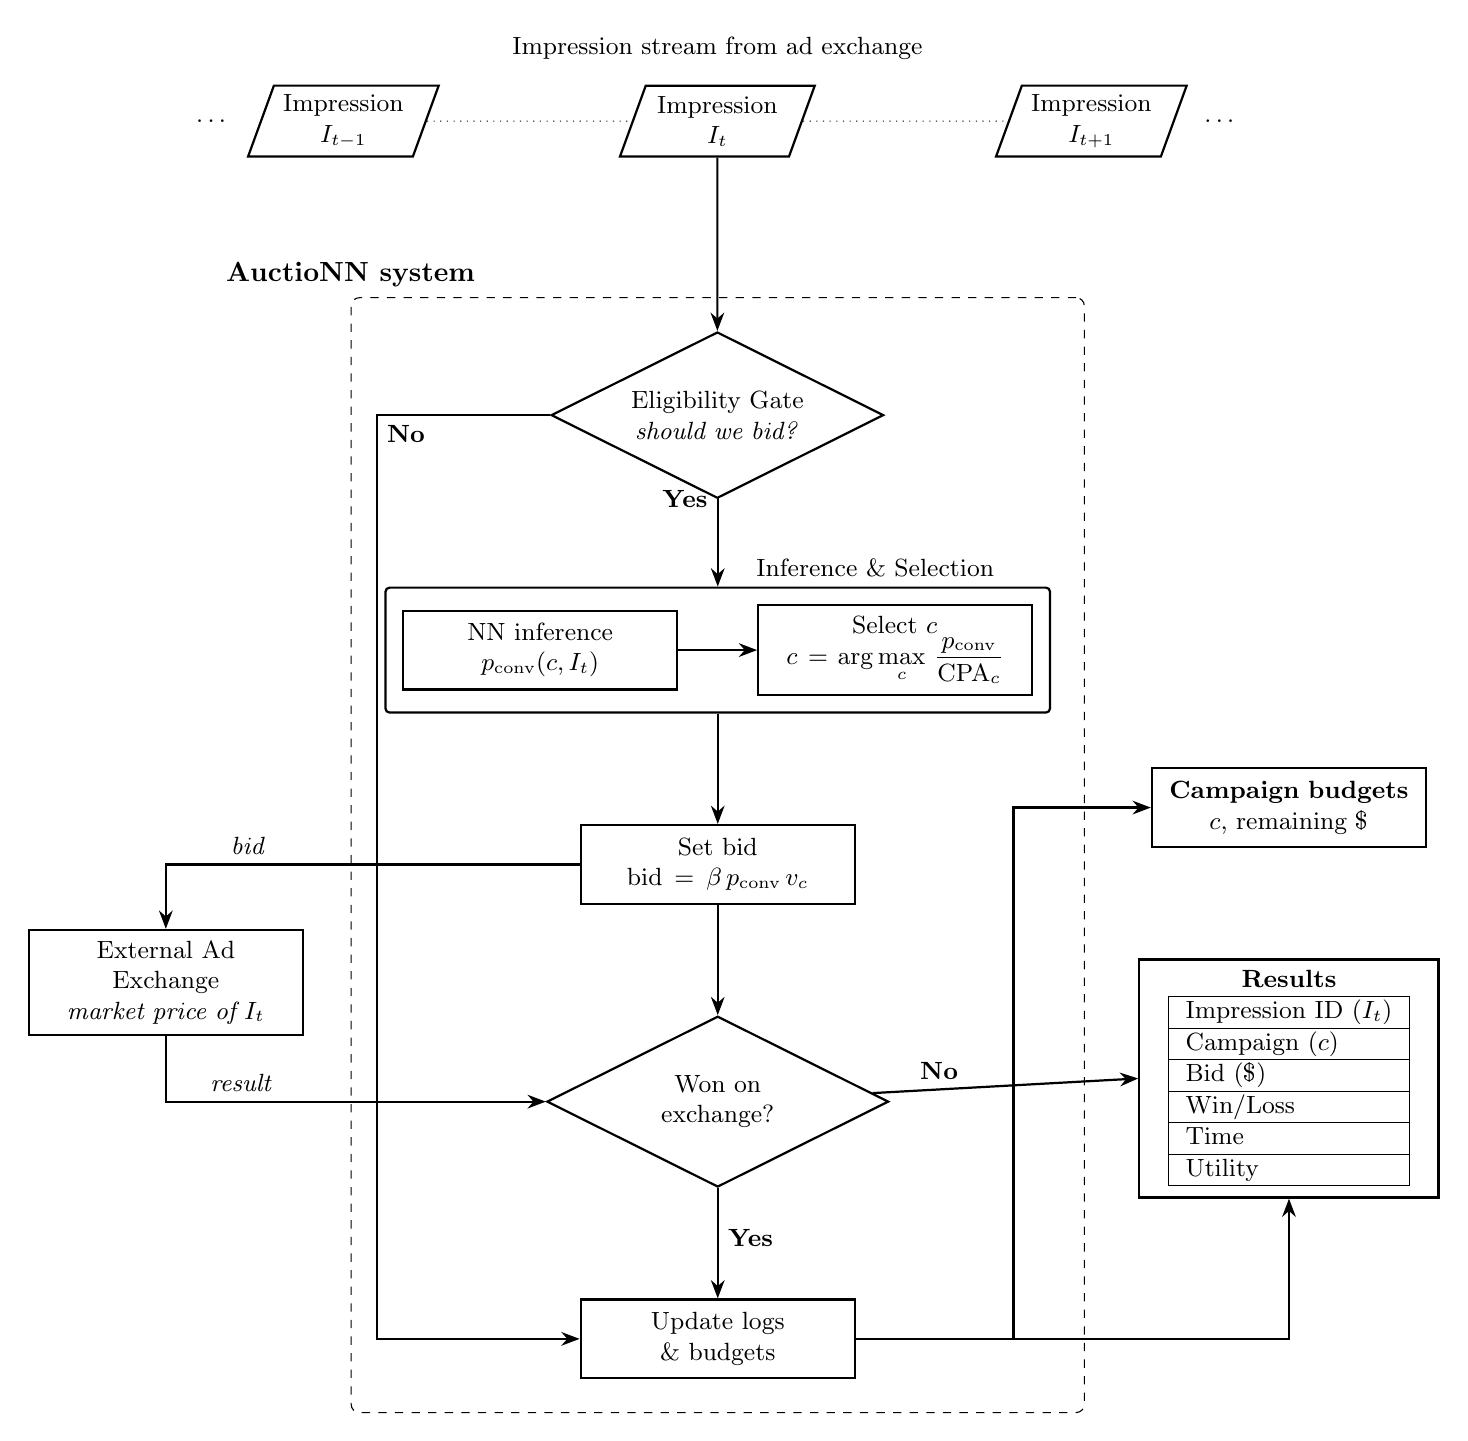
\begin{tikzpicture}[
      font=\small,
      node distance = 14mm and 26mm,
      >=Stealth,
      line/.style      = {thick,->},
      block/.style     = {rectangle, draw, thick, align=center,
        text width=32mm, inner sep=4pt,
      minimum height=10mm},
      decision/.style  = {diamond, draw, thick, align=center,
      aspect=2, inner sep=1pt, text width=28mm},
      io/.style        = {trapezium, draw, thick, align=center,
        trapezium left angle=70, trapezium right angle=110,
      minimum width=22mm, minimum height=9mm},
      dashedBox/.style = {draw, dashed, rounded corners=3pt, inner sep=12pt},
      compoundBox/.style = {rectangle, draw, thick, rounded corners=1.5pt,
      inner sep=6pt}
    ]

    % ---------------- impression stream ----------------
    \node[io]                       (impPrev) {Impression\\$I_{t-1}$};
    \node[io, right=of impPrev]     (imp)     {Impression\\$I_t$};
    \node[io, right=of imp]         (impNext) {Impression\\$I_{t+1}$};

    \node[above=2mm of imp, font=\small] (streamLabel)
    {Impression stream from ad exchange};

    \draw[dotted] (impPrev) -- (imp) -- (impNext);
    \node[right=0.25cm of impNext] (dotsR) {$\dots$};
    \node[left=0.25cm of impPrev]  (dotsL) {$\dots$};

    % ---------------- decision loop ----------------
    \node[decision, below=22mm of imp]  (gate)
    {Eligibility Gate\\\textit{should we bid?}};

    % --- compound Inference + Selection block ---
    % sub-blocks
    \node[block, below=of gate, xshift=-2.25cm]         (nn)
    {NN inference\\$p_{\text{conv}}(c,I_t)$};
    \node[block, right=10mm of nn]      (argmax)
    {Select $c^{\*}$\\$\displaystyle
    c^{\*}=\arg\max_{c}\,\frac{p_{\text{conv}}}{\text{CPA}_c}$};
    % enclosing box
    \node[compoundBox, fit=(nn)(argmax), label=north:{ \hspace{4cm}Inference
    \& Selection}]
    (infsel) {};

    % remaining blocks
    \node[block, below=of infsel] (bid)
    {Set bid\\$\text{bid}=\beta\,p_{\text{conv}}\,v_c$};
    \node[decision, below=of bid] (win?)
    {Won on\\exchange?};
    \node[block, below=of win?]   (update)
    {Update logs\\\& budgets};

    % dashed container around whole logic
    \node[dashedBox, fit=(gate)(infsel)(bid)(win?)(update)] (sysbox){};
    \node[above=0pt of sysbox.north west, font=\bfseries] {AuctioNN system};

    % ---------------- external tables ----------------
    \node[block, right=60mm of nn, yshift=-2cm] (budget)
    {\textbf{Campaign budgets}\\$c$, remaining \$};
    \node[block, below=of budget, minimum width=38mm,
    minimum height=23mm] (results) {
      \textbf{Results}\\[2pt]
      \begin{tabular}{|l|}
        \hline Impression ID ($I_t$)\\ \hline
        Campaign ($c$)\\ \hline
        Bid (\$)\\ \hline
        Win/Loss\\ \hline
        Time\\ \hline
        Utility\\ \hline
    \end{tabular}};

    \node[block, left=35mm of bid, yshift=-15mm] (exchange)
    {External Ad Exchange\\\textit{market price of $I_t$}};

    % ---------------- arrows (main flow) -------------
    \draw[line] (imp) -- (gate.north);

    \draw[line] (gate.south) -| node[left]{\bfseries
    Yes} (infsel.north);
    \draw[line] (nn) -- (argmax);
    \draw[line] (infsel.south) -- (bid.north);

    \draw[line] (bid.south) -- (win?.north);

    \draw[line] (win?.south) -- node[right, yshift=2pt]{\bfseries Yes} (update);

    % ---------------- arrows (side paths) ------------
    % No-bid branch
    \draw[line] (gate.west) -- ++(-22mm,0) |- node[right,
    pos=0.01]{\bfseries No}
    (update.west);

    % bid to exchange
    \draw[line] (bid.west) -| node[above, pos=0.4]{\textit{bid}}
    (exchange.north);
    % result back
    \draw[line] (exchange.south) |- node[above, pos=0.6]{\textit{result}}
    (win?.west);

    % win? -> results  (No branch)
    \draw[line] (win?) -- node[near start, above]{\bfseries No}
    (results.west);

    % update -> budgets & results
    \draw[line] (update.east) -- ++(20mm,0) |- (budget.west);
    \draw[line] (update.east) -- ++(10mm,0) -| (results.south);

  \end{tikzpicture}
  \caption{Fully connected block diagram of AuctioNN’s
    \emph{per-impression} decision loop, emphasising the continuous stream
    of impressions \(I_{t-1}, I_t, I_{t+1}, \dots\).  The compound
    \emph{Inference \& Selection} stage first scores every campaign with a
    neural network and then chooses \(c^{\*}\) via the displayed arg-max
  rule.}
  \label{fig:auctionn-loop-final}
\end{figure}
\newpage

\vspace{-0.5em}
\section{Neural Model}\label{sec:nn}
\paragraph{Objective.}  Estimate conversion probability conditioned
on both the \emph{impression} and the \emph{campaign}.  This is
analogous to a contextual click-through-rate model but with a conversion label.

\paragraph{Feature vector.}
\begin{itemize}
  \item Categorical embeddings: device type, operating system, DMA,
    and campaign~ID.
  \item Temporal features: hour-of-day and day-of-week encoded as
    sine/cosine pairs.
  \item Continuous exposure feature: current $\mathrm{ad\_stock}$
    (per-user, per-campaign).
\end{itemize}

\paragraph{Architecture.}
Two fully connected layers (128\,\(\rightarrow\) 64) with ReLU
activations, followed by a sigmoid output; $\approx$\;55\,k
parameters.  Exported as TorchScript for \(\le\)\;1 ms inference on
an Apple~M2 core.

\paragraph{Training.}
Binary cross-entropy on historical (impression, conversion) pairs.
Severe class imbalance ($\mathcal{O}(10^{-3})$ converters) is
mitigated via positive-class weighting and mini-batch stratification.
The data pipeline materialises a 7-day attribution window (see
§\ref{sec:openq}).

\section{Evaluation Methodology}\label{sec:evaluation}
We benchmark three policies:

\begin{enumerate}
  \item \textbf{Random}—bid a constant \$1 CPM on a random eligible campaign.
  \item \textbf{Heuristic}—industry default: bid proportional to
    campaign value, ignoring $p_{\mathrm{conv}}$.
  \item \textbf{AuctioNN (proposed)}—full decision loop of
    §\ref{sec:decisionloop}.
\end{enumerate}

\subsection{Success Metrics}
\begin{itemize}
  \item \textbf{Marginal CPA}
    (\(\Delta\)Spend\(/\)\(\Delta\)Conversions) relative to baseline.
  \item \textbf{Total conversions} aggregated across all campaigns.
  \item \textbf{Revenue uplift} (= advertiser value – media cost).
  \item \textbf{Pacing error}:
    $|\mathrm{actual\;spend}-\mathrm{planned\;spend}|/\mathrm{planned\;spend}\le0.05$.
  \item \textbf{Latency}: distributive
    $p_{95}\le\SI{2}{\milli\second}$ per impression on a MacBook
    M-series laptop.
\end{itemize}

\section{Implementation Notes}

\section{Open Questions and Future Work}\label{sec:openq}

\section{Conclusion}
AuctioNN provides a controlled environment to test whether modern ML
can simultaneously optimise CPA, satisfy campaign obligations, and
execute within the harsh latency limits of real-time bidding.  The
architecture is intentionally minimal yet extensible, enabling
rigorous \emph{ablation studies} of every engineering choice—from
eligibility gates to neural features to bid shading policies.

% ----------------------------------------------------------------------
\bibliographystyle{plain}
\bibliography{auctionn}
\end{document}
